% A skeleton file for producing Computer Engineering reports
% https://kgcoe-git.rit.edu/jgm6496/KGCOEReport_template

\documentclass[CMPE]{KGCOEReport}

% The following should be changed to represent your personal information
\newcommand{\classCode}{CMPE 160}  % 4 char code with number
\newcommand{\name}{Andrei Tumbar}
\newcommand{\LabSectionNum}{4}
\newcommand{\LabInstructor}{Mr.\ Byers}	% The slash is to tell LaTeX that the period is between words
												% not sentences so it spaces correctly. It won't appear in the
												% final pdf
\newcommand{\TAs}{Sam Myers \\ Kobe Balin \\ Georgi Thomas}
\newcommand{\LectureSectionNum}{2}
\newcommand{\LectureInstructor}{Mr.\ Cliver}
\newcommand{\exerciseNumber}{1}
\newcommand{\exerciseDescription}{Electrical and Logical Characteristics of Gates}
\newcommand{\dateDone}{January 30th}
\newcommand{\dateSubmitted}{February 6th}

\graphicspath{{./lab3_media/}}

\usepackage{circuitikz}
\usepackage{tikz}
\usepackage{multirow}
\usepackage{titlesec}
\usepackage{float}
\usepackage{pgfplots, pgfplotstable}

\setcounter{secnumdepth}{2}

\def\coord(#1){coordinate(#1)}
\def\coord(#1){node[circle, red, draw, inner sep=1pt,pin={[red, overlay, inner sep=0.5pt, font=\tiny, pin distance=0.1cm, pin edge={red, overlay,}]45:#1}](#1){}}
\def\coordd(#1){node[circle, red, draw, inner sep=1pt,pin={[red, overlay, inner sep=0.5pt, font=\tiny, pin distance=0.1cm, pin edge={red, overlay,}]-45:#1}](#1){}}

\begin{document}
\maketitle

\section*{Abstract}
In the laboratory exercise, the logical characteristics of basic gates and measurments regarding the delay of a inverter oscillator were studied. In part one, switches from the input of the previous lab exercise were connected to three different ICs for testing. These two switches acted as inputs for the gates on the ICs. Measurements were taken for a two input NAND (74LS00), OR (74LS32), and an XOR (74LS86) gate. The purpose of this was to give students experience in using an IC's circuit diagram and wiring the IC to an LED. \par 
In the second part of this lab exercise, the time delay associated with a series of inverter gates was investigated. Five inverters were wired in a series and the delay after each inverter was probed and recorded. Measurements for each inverter delay was taken along with the period of oscillation.

\section*{Design Methodology}

\subsection*{Part One}
In part one of this lab, three different IC's werer tested using two switches from the previous exercise as input and one of the LEDs as output. \par
NAND, OR, and XOR IC were used. Because input, output, \(V_c\), and ground were located on the same relative pins on all three ICs, each IC could be swapped for the next type.

\begin{figure}[h]
\centering
\begin{circuitikz}[american, ]
	\ctikzset{multipoles/thickness=4}
	\ctikzset{multipoles/external pins thickness=2}	
	
	\draw (0,0) node[dipchip,
		num pins=14,
		external pins width=0.3,
		external pad fraction=4 ](C){IC};
	
	\draw (0,4) node[vcc](VCC){\(V_{CC} = 5\,V\)};
   	\draw (C.pin 14) -- ++(0.2,0) -- ++(0,0.5) -- ++(-1.45,0)  -- (VCC){};
   	\draw (C.pin 7) -- ++ (-4,0) node[ground, rotate=-90](gnd){};
   	\draw (C.pin 2) to[short, -*] ++(-2.94,0) -- (-4.2,3.5) to[R, bipoles/length=.8cm] ++(2,0) -- (0,3.5)  to[short, -*] ++ (0,0) (-4.2,1.2) to[ospst] ++(0,-2.87) to[short, -*] ++(0,0);
   	
   	\draw (C.pin 1) to[short, -*] ++(-2.44,0) -- ++(0,1.2) to[R, bipoles/length=.8cm] ++(2,0) -- (0,2.88)  to[short, -*] ++ (0,0) (-3.7, 1.8) -- (-3.7,1.2) to[ospst] ++(0,-2.87) to[short, -*] ++(0,0);
   	
   	\draw (C.pin 3) -- ++(-1,0) node[label={[font=\footnotesize]below:To LED}]{} to[short, -*] ++(0,0);

\end{circuitikz}

\caption{Example wiring for IC}
\label{fig:IC}
\end{figure}

Figure \ref{fig:IC} depicts switches to represent the input circuit from the last labs exercise. A resistor is placed between the power supply and the switch so that when the switch is closed, there is no short circuit between the ground and voltage supply. When the switch is open, $5\,V$ is supplied to the IC therefore inputing an ON signal to the device. When the switch is closed however, the wire is connected to ground therefore putting the wire at $0\,V$ relative to ground.
A record of the output voltage (PIN 3) from each IC on every input combination as well as the results on the output LED were taken.

\subsection*{Part Two}
In part two, delay and oscillation period associated with inverters were investigated. Five inverters were wired in a series with a space for a probe to record the voltage on each node. The order that the inverters were connected proved unimportant as long as the final connection looped back to the first inverter.

\begin{figure}[h]
\centering
\begin{circuitikz}[american, ]
	\ctikzset{multipoles/thickness=4}
	\ctikzset{multipoles/external pins thickness=2}	
	
	\draw (0,0) node[american not port](i1){};
	\draw (2,0) node[american not port](i2){};
	\draw (4,0) node[american not port](i3){};
	\draw (6,0) node[american not port](i4){};
	\draw (8,0) node[american not port](i5){};
	
	\draw (i1.out) -- (i2.in);
	\draw (i2.out) -- (i3.in);
	\draw (i3.out) -- (i4.in);
	\draw (i4.out) -- (i5.in);
	\draw (i5.out) -- ++(1, 0) -- ++(0, -1.5) -- (-1.8, -1.5) -- ++(0, 1.5) -- (i1.in);

\end{circuitikz}

\caption{Circuit diagram for the inverter oscillator}
\label{fig:OSC}
\end{figure}

Figure \ref{fig:OSC} shows the circuit diagram for the inverter oscillator. The CH1 probe was placed on the node before the first inverter. This probe acted as the reference measurement which subsequent measurements would be based off of. The CH2 probe was placed after each of the inverters and a delay measurement was taken. Both probes were grounded prior to any measurement. Each measurement needed to take in account the logical value of each probe. Because the the first probe was set in front of a rising inverter, the possible measurements were: rising to falling or rising to rising. Four measurements where taken after each inverter to find the total gate propagation. 

\section*{Results and Analysis}

\subsection*{Part One}
\subsubsection{NAND gate}

The first gate that was tested was the NAND 74LS00N IC. By connecting the multimeter to the output node measurements were taken. Table \ref{tab:NAND} shows the results of the mesurements taken for the NAND gate.

\begin{table}[h]
\renewcommand{\arraystretch}{1.2}
\caption{Measurements of a two input NAND gate circuit}
\begin{center}
\begin{tabular}{|c|c|c|c|c|c|}
\hline
Switch 1 Position & Switch 2 Position & $V_{in,1}$ (V) & $V_{in,2}$ (V) & $V_{out}$ (V) & LED (on/off)\\\hline

Closed & Closed & 0 & 0 & 4.1  & ON \\\hline
Closed & Open   & 0 & 5 & 4.1  & ON \\\hline
Open   & Closed & 5 & 0 & 4.1  & ON \\\hline
Open   & Open   & 5 & 5 & 0.27 & OFF \\\hline
\multicolumn{5}{|r|}{Logical function of gate: } & NAND  \\\hline
\multicolumn{5}{|r|}{Lab kit part number for gate: } & 74LS00N  \\\hline

\end{tabular}
\end{center}
\label{tab:NAND}
\end{table}

Table \ref{tab:NAND} shows the input and output voltages measured in the NAND gate. The inputs are either $0\,V$ or $5\,V$ depending on the position of the switch. When the switch is closed, the input is connected to ground therefore setting the potential of the input to $0\,V$. Conversely, when the switch is open, the potential of the input node is near $5\,V$. It is near $5\,V$ because there is still a resistor in series before. Table 1's output voltages conform to the electrical characteristics described on the IC's datasheet. The high output voltage is described to have a minimum value of $2.7\,V$, at $4.1\,V$ this easily meets the requirement. For the low output voltage, the datasheet describes a maximum value of $0.5\,V$ with a typical value of $0.35\,V$. The measured voltage was $0.27\,V$ which is close to that described on the sheet. In regards to the output of the circuit, because it was a NAND gate, the only time the LED should be OFF is when both inputs are logical 1. The expected result was observed.


\subsubsection{OR gate}
The next gate that was tested was the two input OR gate. The 74LS32N chip was used to take measurements. Table \ref{tab:OR} shows the measurements taken in this section of the exercise.

\begin{table}[h]
\renewcommand{\arraystretch}{1.2}
\caption{Measurements of a two input OR gate circuit}
\begin{center}
\begin{tabular}{|c|c|c|c|c|c|}
\hline
Switch 1 Position & Switch 2 Position & $V_{in,1}$ (V) & $V_{in,2}$ (V) & $V_{out}$ (V) & LED (on/off)\\\hline

Closed & Closed & 0 & 0 & 0.09  & OFF \\\hline
Closed & Open   & 0 & 5 & 4.07  & ON \\\hline
Open   & Closed & 5 & 0 & 4.07  & ON \\\hline
Open   & Open   & 5 & 5 & 4.07 & ON \\\hline
\multicolumn{5}{|r|}{Logical function of gate: } & OR  \\\hline
\multicolumn{5}{|r|}{Lab kit part number for gate: } & 74LS32N  \\\hline

\end{tabular}
\end{center}
\label{tab:OR}
\end{table}

The input circuit and resultant measurements in Table \ref{tab:OR} for this circuit are the same because nothing was changed from there. The outputs, however, are different because this gate conforms to a different range of values. The typical and minimum output voltages on the 74LS32 gate are $3.4\,V$ and $2.7\,V$ respectively. The measured voltage was $4.07\,V$ on all logical 1 outputs. This value is well within the limits. The logical 0 output voltage was measured to be $0.09\,V$. With a listed maximum voltage of $0.4\,V$, this measurement is also well within the limits. The LED is only OFF when both inputs are OFF. This is consistent with the logical function of the OR gate.

\subsubsection{XOR gate}
The XOR (74LS86) gate is meant to output a logical 1 when the two inputs are inequivalent. Table \ref{tab:XOR} shows the measurements taken for this IC.

\begin{table}[h]
\renewcommand{\arraystretch}{1.2}
\caption{Measurements of a two input XOR gate circuit}
\begin{center}
\begin{tabular}{|c|c|c|c|c|c|}
\hline
Switch 1 Position & Switch 2 Position & $V_{in,1}$ (V) & $V_{in,2}$ (V) & $V_{out}$ (V) & LED (on/off)\\\hline

Closed & Closed & 0 & 0 & 0.151 & OFF \\\hline
Closed & Open   & 0 & 5 & 4.1   & ON \\\hline
Open   & Closed & 5 & 0 & 4.1   & ON \\\hline
Open   & Open   & 5 & 5 & 0.163 & OFF \\\hline
\multicolumn{5}{|r|}{Logical function of gate: } & XOR  \\\hline
\multicolumn{5}{|r|}{Lab kit part number for gate: } & 74LS86AN  \\\hline

\end{tabular}
\end{center}
\label{tab:XOR}
\end{table}

Again, inputs in Table \ref{tab:XOR} are equivalent to the other two sets of measurements. The measured low outputs were under the maximum logical 0 voltage of $0.5\,V$. The measured high outputs of $4.1\,V$ were well above the minimum voltage for logical 1 of $2.7\,V$. The LEDs were expected to be ON when the input signals have opposite logical states. This same expected output was observed in Table \ref{tab:XOR}.


\subsection*{Part Two}

Four different screen captures from the oscilliscope were taken on each of the nodes to show the delay propagation. Images taken from oscilliscope were inverted to make better use of colors and contrast.


\begin{figure}[H]
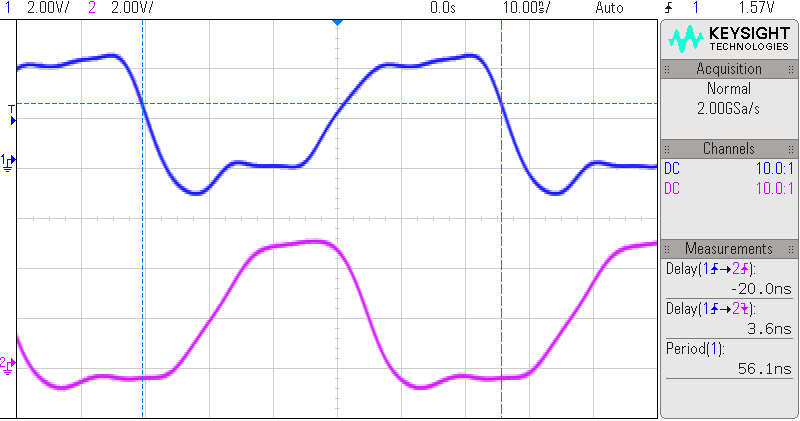
\includegraphics[width=\textwidth]{fig1}
\label{fig:osc-1}
\caption{Oscilloscope measurement with one gate of delay} 
\end{figure}

\begin{figure}[H]
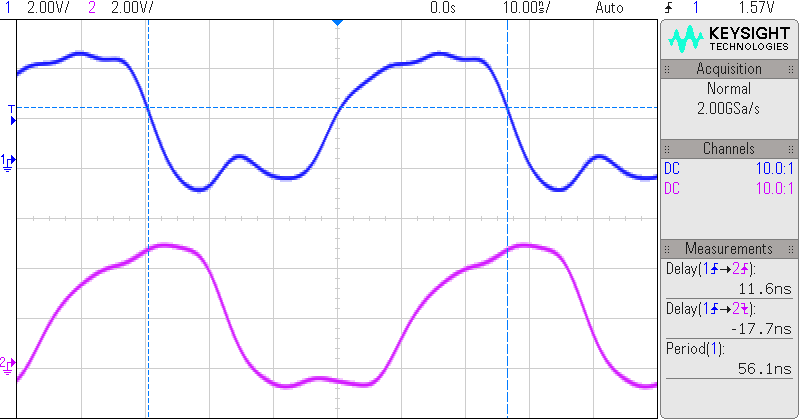
\includegraphics[width=\textwidth]{fig2}
\label{fig:osc-2}
\caption{Oscilloscope measurement with two gates of delay} 
\end{figure}

\begin{figure}[H]
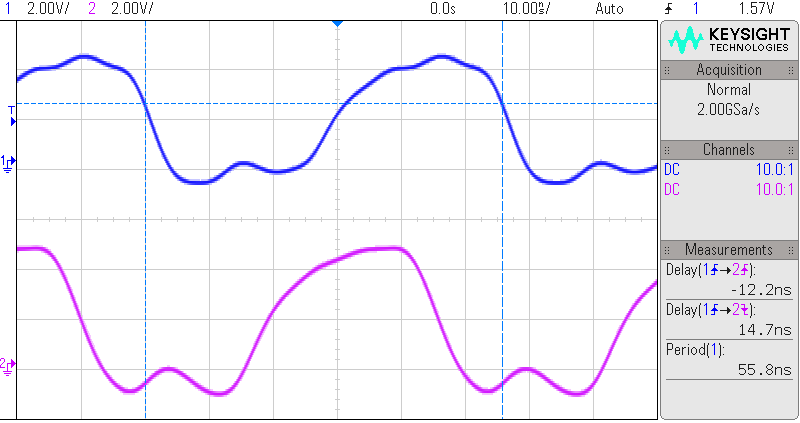
\includegraphics[width=\textwidth]{fig3}
\label{fig:osc-3}
\caption{Oscilloscope measurement with three gates of delay} 
\end{figure}

\begin{figure}[H]
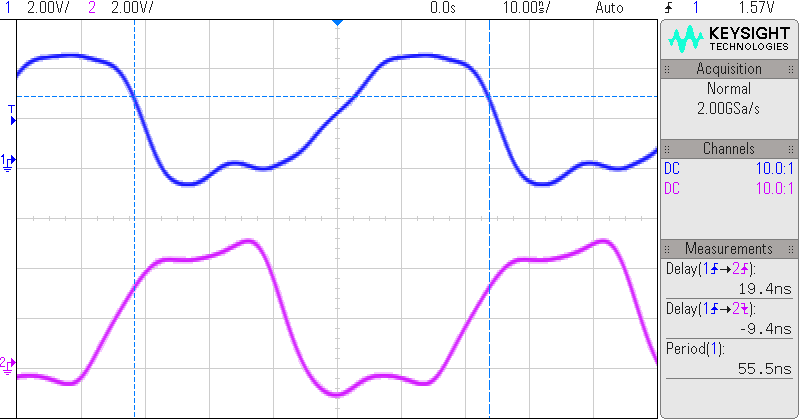
\includegraphics[width=\textwidth]{fig4}
\label{fig:osc-4}
\caption{Oscilloscope measurement with four gates of delay} 
\end{figure}

Screen captures from the oscilliscope show the voltages relative to ground on each of the nodes inbetween the gates over time. They oscillate with a period of about $55\,ns$ because the circuit consists of an odd number of inverters.\par


Four measurements were taken in Table \ref{tab:INV} corresponding to the total delay propagation from the reference point to that gate.

\begin{table}[h]
\renewcommand{\arraystretch}{1.2}
\caption{Effect of propagation delay}
\begin{center}
\begin{tabular}{|c|c|c|}
\hline

74LS04 & Number of Gates & Propagation Delay \\
(pin to pin) & of Delay & (ns)\\\hline

2 to 4 (rising to falling) & 1 & 3.4\\\hline
2 to 6 (rising to rising) & 2 & 11.7\\\hline
2 to 12 (rising to falling) & 3 & 14.7\\\hline
2 to 10 (rising to rising) & 4 & 19.4\\\hline
\multicolumn{2}{|r|}{Period: } & 55.6  \\\hline

\end{tabular}
\end{center}
\label{tab:INV}
\end{table}

The delay propagation shown in Table \ref{tab:INV} shows that rising to falling vs rising to rising inversions have different values associated. If the direction of inversion is ignored, the average delay for each gate is $4.55\,ns$. When taking account of the direction of inversion, the average rising to falling delay was $3.25\,ns$ whereas the rising to rising was $5.8\,ns$. The period measured was $55.8\,ns$. The square wave oscillated on the figures 3\,-6 because there was an odd number of inverters in the circuit. After the signal ran through all of the inverters the original low signal inverted itself. Therefore the first oscillator would have a different input signal. If an even number of inverters were used, the probes would display no change in potential over time.

The measured period refers to the period of oscillation in the reference probe. The total time it would take to switch the logical value on the reference node would be $19.4 + one\ inverter\ delay$. This is because the delay for four gates was $19.4\,ns$, however, there are five inverter gates. If the average gate delay of an inverter ($5\,ns$) was added to the total delay measured, the half period delay would be around $23.2\,ns$. The full period would be calculated to around $46.4\,ns$. However, the measured period was $55.8\,ns$ meaning that the final inverter had a delay of $8.4\,ns$. This number is still within the range on the datasheet of the chip.

\pgfplotstableread{
X Y
0 0
1 3.4
2 11.7
3 14.7
4 19.4
}\datatable

\begin{figure}[H]
\begin{center}
\begin{tikzpicture}
\begin{axis}[
    xlabel={Number of gates},
    ylabel={Propgation Delay ($ns$)},
    xmin=0, xmax=5,
    ymin=0, ymax=20,
    xtick={0,1,2,3,4,5},
    ytick={0,2.5,5,7.5,10,12.5,15,17.5,20},
    legend pos=north west,
    ymajorgrids=true,
    xmajorgrids=true,
    grid style=dashed,
]

\addplot[mark = *] plot [error bars/.cd, y dir = both, y explicit] table[x=X, y=Y] {\datatable};

\end{axis}
\end{tikzpicture}

\caption{Graphed delay propagation vs number of gates used}
\label{fig:delay}
\end{center}
\end{figure}

Figure \ref{fig:delay} shows the delay propagation from each inverter. The odd x-values indicate a rising to falling measurement while the even numbers read a rising to rising measurement. It can clearly be seen that the rising to falling delays are shorted than the rising to rising. This can be seen in the slopes between the ploted points. The slope from even to odd numbers is far lower than that of odd to even numbers.


\section*{Conclusion}

This laboratory exercise investigated the logical and electrical properies of gates by testing a variety of different two-input logical gate chips. In the second part, the delay propagation and period of oscillation associated with a chain of inverter gates was investigated. A $55.8\,ns$ period of oscillation was observed for a 5-inverter chain. The purpose of this lab was to clarify how chips and their datasheets are used within circuit design. 

\section*{Questions}

\begin{enumerate}
  \item What are these voltage values for the 74LS27
  \begin{enumerate}
  	\item Minimum input voltage for logic 1
  	
  	\textbf{2 V}
  	
  	\item Maximum input voltage for logic 0
  	
  	\textbf{0.7 V}
  	
  	\item Minimum output voltage for logic 1
  	
  	\textbf{2.7 V}
  \end{enumerate}
  
  \item Define propagation delay, and discuss how it impacts the output a gate. Why is it a consideration in digital designs?
  
  Propagation delay is the total time it takes for a circuit to provide an output signal given a set of input signals. Delays are propagated through the use of multiple gates because each gate has a delay associated with it. It is important to consider this delay in digital designs because an output value should not be read until the maximum delay from any path in the circuit has elapsed.
  
  \item Design an XOR gate using 74LS08 (2-input AND), a 74LS04 (6-inverter) and a 74LS32(2-input OR). 
\end{enumerate}

\begin{figure}[h]
\centering
\begin{circuitikz}[american, ]
	\ctikzset{multipoles/thickness=4}
	\ctikzset{multipoles/external pins thickness=2}	
	
	
	%\draw [help lines] (-4,4) grid (4,-8);%
	
	\node [label={[label distance=-1.4cm,text depth=0em,rotate=-90]right:74LS08 (AND)}] at (-0.13,0) {};
	
	\node [label={[label distance=-1.3cm,text depth=0em,rotate=-90]right:74LS32 (OR)}] at (-0.13,-5) {};
	
	\node [label={[label distance=-1.5cm,text depth=0em,rotate=-90]right:74LS04 (NOT)}] at (-4.53,0) {};
	
	\draw (0,0) node[dipchip,
		num pins=14,
		external pins width=0.3,
		external pad fraction=4 ](AND){};
	
	\draw (0,-5) node[dipchip,
		num pins=14,
		external pins width=0.3,
		external pad fraction=4 ](OR){};
		
	\draw (-4.4,0) node[dipchip,
		num pins=14,
		external pins width=0.3,
		external pad fraction=4 ](NOT){};
	
	
	\draw (AND.pin 1) -| (-2,3.4)   node (B) [label=S2]{} to [short, *-] ++(0,0);
	\draw (NOT.pin 13) -| (-2.5,3.4) node (A) [label=S1]{} to [short, *-] ++(0,0);
	\draw (NOT.pin 12) -- ++(0.8,0)  |- (AND.pin 2);
	\draw (AND.pin 3)  -- ++(-0.4,0) |- (OR.pin 1);
	
	\draw (-2,1.68) node (c1) {} to [short, -*] ++(0,0);
	\draw (-2,1.68) |- (NOT.pin 11);
	
	\draw (NOT.pin 10) |- (AND.pin 5);
	\draw (NOT.pin 13) ++ (0.3,0) node (c2) {} to[short, *-] ++(0,-1.5) -- ++ (1.4,0) |- (AND.pin 4);
	
	\draw (AND.pin 6) -- ++ (-0.7,0) |- (OR.pin 2);
	\draw (OR.pin 3) -- ++ (-2,0) node [label=L1]{} to [short, -*] ++(0,0);
	
	\draw (-4.4,-3) node[ground, rotate=180](GND){};
	\draw (NOT.pin 7) -- ++(-0.4,0) |- (GND.center);
	\draw (OR.pin 7) -| (GND.center);
	\draw (AND.pin 7) -- ++(-1,0) |- (GND.center) to[short, *-] ++(0,0);
	\draw (NOT.pin 14) -- ++(0.3,0) -- ++(0,0.8) -- ++(4.5,0) node(VC){}  |- (AND.pin 14);
	\draw (OR.pin 14) -- ++(0.4,0) |- (AND.pin 14);
	\draw (AND.pin 14) to[short, -*] ++(0.4,0) -| ++(0.4,1) node[vcc]{$V_{CC}$};
	
	

\end{circuitikz}

\caption{Circuit for 2-input XOR}
\label{fig:XOR_IMPL}
\end{figure}

\end{document}
